\documentclass[letterpaper,12pt,fleqn]{article}
\usepackage{matharticle}
\usepackage{polynom}
\pagestyle{plain}
\begin{document}

\begin{center}
\Large Math-19 Homework \#10 Solutions
\end{center}

\vspace{0.5in}

\underline{Problems}

\begin{enumerate}
\item Divide $8x^4+4x^3+6x^2$ by $2x^2+1$. Show \emph{all} work and state your
  final answer in division algorithm form.

  This is a bit hard to typeset properly. The package that does this
  automatically doesn't put in the fillers and applies the minus sign, but
  you get the idea.

  $\polylongdiv{8x^4+4x^3+6x^2+0x+0}{2x^2+0x+1}$

  So, in DA form:

  $8x^4+4x^3+6x^2=(2x^2+1)(4x^2+2x+1)-2x-1=(2x^2+1)(4x^2+2x+1)-(2x+1)$

\item Consider the following graph of a polynomial:

  \begin{tikzpicture}
    \draw (-4,0) -- (4,0);
    \draw (0,-4) -- (0,4);
    \draw [domain=-2.3:2.3] plot ({\x},{0.5*(\x-2)*(\x-1)*(\x+1)*(\x+2)});
    \node [draw,circle,fill,scale=0.5] at (2,0) {};
    \node [below right] at (2,0) {$(2,0)$};
    \node [draw,circle,fill,scale=0.5] at (-1/2,45/32) {};
    \node [above left] at (-1/2,45/32) {$(-\frac{1}{2},\frac{3}{2})$};
  \end{tikzpicture}

  \begin{enumerate}
  \item What is the remainder when the polynomial is divided by $(x-2)$?

    By the remainder theorem, $p(2)=0=r$.

    $r=0$
    
  \item What is the remainder when the polynomial is divided by
    $\left(x+\frac{1}{2}\right)$?

    By the remainder theorem, $p\left(-\frac{1}{2}\right)=\frac{3}{2}=r$.

    $r=\frac{3}{2}$
    
  \end{enumerate}

\item Consider the polynomial function:
  \[y=4x^7-4x^6-15x^5+16x^4-4x^3\]
  \begin{enumerate}
  \item Factor completely. You must show \emph{all} work (clearly), including
    selection of candidates, determining which candidates are roots, and
    successively dividing out factors. Be sure to clearly state your final
    factorized form.

    First, factor out an $x^2$ and then work on what is left.

    $y=x^3(4x^4-4x^3-15x^2+16x-4)$

    Now, identify candidates for $p_1(x)=4x^4-4x^3-15x^2+16x-4$:

    $a_0=-4$ and $a_n=4$

    $p=\pm1,\pm2,\pm4$ \\
    $q=\pm1,\pm2,\pm4$

    $\frac{p}{q}: \pm1,\pm2,\pm4,\pm\frac{1}{2},\pm\frac{1}{4}$

    Use the remainder theorem to find a zero:

    $p_1(1)=4-4-15+16-4\ne0$ \\
    $p_1(-1)=4+4-15-16-4\ne0$ \\
    $p_1(2)=64-32-60+32-4=0$

    Found one. Now divide by $x-2$:

    $\polylongdiv{4x^4-4x^3-15x^2+16x-4}{x-2}$

    Now we have:

    $p(x)=x^3(x-2)(4x^3+4x^2-7x+2)$

    Get new candidates for: $p_2(x)=4x^3+4x^2-7x+2$

    $p=\pm1,\pm2$ \\
    $q=\pm1,\pm2,\pm4$

    $\frac{p}{q}: \pm1,\pm2,\pm\frac{1}{2},\pm\frac{1}{4}$

    We already eliminated $\pm1$ is the previous step; however, we need to
    retry $2$, just in case it is a repeated root:

    $p_2(2)=32+16-14+2\ne0$
    $p_2(-2)=-32+16+14+2=0$

    So divide out $x+2$:

    $\polylongdiv{4x^3+4x^2-7x+2}{x+2}$

    Now:

    $p(x)=x^3(x-2)(x+2)(4x^2-4x+1)$

    The last quadratic factors easily and we have the final result:

    $p(x)=x^3(x-2)(x+2)(2x-1)^2$

  \item Sketch the graph. All intercepts must be labeled.

    Here are the zeros and their multiplicities:

    \begin{tabular}{ccc}
      zero & multiplicity & change sign? \\
      \hline
      $-2$ & $1$ & yes \\
      $0$ & $3$ & yes \\
      $\frac{1}{2}$ & $2$ & no \\
      $2$ & $1$ & yes
    \end{tabular}

    This results in the following $x$-intercepts:

    $(-2,0),(0,0),(\frac{1}{2},0),(2,0)$

    And $y$-intercept:

    $(0,0)$

    The leading term is $4x^7$: an odd power and a positive coefficient, so the
    end behavior is like $x^3$:

    \begin{tikzpicture}
      \draw (-5,0) -- (5,0);
      \draw (0,-5) -- (0,5);
      \node [draw,circle,fill,scale=0.5] (x1) at (-2,0) {};
      \node [draw,circle,fill,scale=0.5] (x2) at (0,0) {};
      \node [draw,circle,fill,scale=0.5] (x3) at (1/2,0) {};
      \node [draw,circle,fill,scale=0.5] (x4) at (2,0) {};
      \node [below] at (x1) {$-2$};
      \node [below left] at (x2) {$0$};
      \node [below] at (x3) {$\frac{1}{2}$};
      \node [below] at (x4) {$2$};
      \draw [smooth] plot coordinates {
        (-3,-5) (-2,0) (-1.25,4) (-0.25,0.25) (0,0)
        (0.25,-0.5) (1/2,0) (5/4,-3) (2,0) (3,5)
      };
    \end{tikzpicture}

    Note the shape at $(0,0)$ which is a point of inflection.

  \end{enumerate}

\item Consider the rational function:
  \[y=\frac{3(x-1)^3(x^2-9)}{(2x^3-6x^2)(x^2-4)}\]
  \begin{enumerate}
  \item What are the zeros?

    First factor the numerator and denominator:

    $y=\frac{3(x-1)^3(x+3)(x-3)}{2x^2(x-3)(x+2)(x-2)}$

    Cancel the $x-3$, but remember that we may need to make a hole at $x=3$:
    
    $y=\frac{3(x-1)^3(x+3)}{2x^2(x+2)(x-2)}$

    Now, the zeros are obviously at $x=1,-3$

  \item What are the poles?

    $x=0,\pm2$
    
  \item What is the y-intercept?

    Note that $x=0$ is a pole, so there is no y-intercept.
    
  \item What is the horizontal asymptote?

    Both the numerator and denominator are of degree $4$, so the horizontal
    asymptote is the ratio of the leading coefficients:

    $y=\frac{3}{2}$
    
  \item Sketch the graph. You must label all intercepts, asymptotes, and any
    holes that may occur. All zeros must have the proper shape and the end
    behaviors must be correct.

    The end behavior is a bit tricky. We know that it is asymptotic to
    $y=\frac{3}{2}$; however, we don't know if it approaches from above or
    below. To determine this, we need to expand the numerator and denominator
    and then do long division:

    $y=\frac{3(x^4-6x^2+8x-3)}{2(x^4-4x^2)}$

    $\polylongdiv{x^4-6x^2+8x-3}{x^4-4x^2}$

    $y=\frac{3}{2}\left(1+\frac{-2x^2+8x-3}{x^4-4x^2}\right)=
    \frac{3}{2}\left(1-\frac{2x^2-8x+3}{x^4-4x^2}\right)$

    We need to see how $\frac{2x^2-8x+3}{x^4-4x^2}$ changes sign during the
    end behavior (i.e., past the last zero/pole). If it is $<0$ then the
    graph is above the asymptote. If it is $>0$ then the graph is below the
    asymptote. The numerator doesn't factor nicely, so we will use the
    quadratic formula:

    $x=\frac{8\pm\sqrt{(-8)^2-4(2)(3)}}{2(2)}=
    \frac{8\pm\sqrt{40}}{4}=\frac{4\pm\sqrt{10}}{2}\approx0.4,3.6$

    So we have:

    $y=\frac{3}{2}\left(1-\frac{
      \left(x-\frac{4-\sqrt{10}}{2}\right)
      \left(x-\frac{4+\sqrt{10}}{2}\right)}
    {x^2(x+2)(x-2)}\right)$

    Using the techniques from chapter 1:

    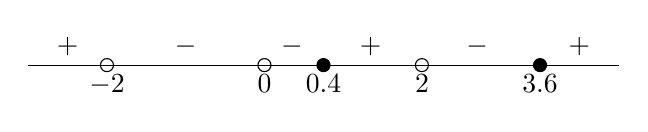
\begin{tikzpicture}
      \draw (-3,0) -- (4.5,0);
      \node [draw,circle,scale=0.5] (x1) at (-2,0) {};
      \node [draw,circle,scale=0.5] (x2) at (0,0) {};
      \node [draw,circle,fill,scale=0.5] (x3) at (0.75,0) {};
      \node [draw,circle,scale=0.5] (x4) at (2,0) {};
      \node [draw,circle,fill,scale=0.5] (x5) at (3.5,0) {};
      \node [below] at (x1) {$-2$};
      \node [below] at (x2) {$0$};
      \node [below] at (x3) {$0.4$};
      \node [below] at (x4) {$2$};
      \node [below] at (x5) {$3.6$};
      \node [above] at (-2.5,0) {$+$};
      \node [above] at (-1,0) {$-$};
      \node [above] at (0.35,0) {$-$};
      \node [above] at (1.35,0) {$+$};
      \node [above] at (2.7,0) {$-$};
      \node [above] at (4,0) {$+$};
    \end{tikzpicture}

    So before $x=-3$ the correction is always positive, and so the graph
    approaches the asymptote from below. But past $x=2$ the correction starts
    off negative and then goes positive after about $x=3.6$. Thus, the graph is
    above the asymptote, crosses at about $x=3.6$, and then approaches from
    below.

    Also, remember to leave a hole at $x=3$. The corresponding $y$ value is:

    $y(3)=\frac{3(8)(6)}{2(9)(5)(1)}=\frac{8}{5}$

    Putting this altogether we have:

    \begin{tikzpicture}
      \draw (-5,0) -- (5,0);
      \draw (0,-10) -- (0,10);
      \node [draw,circle,fill,scale=0.5] (z1) at (-3,0) {};
      \node [draw,circle,fill,scale=0.5] (z2) at (1,0) {};
      \node [below] at (z1) {$-3$};
      \node [below] at (z2) {$1$};
      \draw [dashed] (-2,-10) -- (-2,10);
      \draw [dashed] (2,-10) -- (2,10);
      \node [below right] at (-2,0) {$-2$};
      \node [below left] at (0,0) {$0$};
      \node [below right] at (2,0) {$2$};
      \draw [dashed] (-5,3/2) -- (5,3/2);
      \node [above left] at (0,3/2) {$\frac{3}{2}$};
      \draw [smooth,domain=-5:-2.2] plot ({\x},
            {(3*((\x)^4-6*(\x)^2+8*(\x)-3))/(2*((\x)^4-4*(\x)^2))});
      \draw [smooth,domain=-1.6:-0.69] plot ({\x},
            {(3*((\x)^4-6*(\x)^2+8*(\x)-3))/(2*((\x)^4-4*(\x)^2))});
      \draw [smooth,domain=0.235:1.955] plot ({\x},
            {(3*((\x)^4-6*(\x)^2+8*(\x)-3))/(2*((\x)^4-4*(\x)^2))});
      \draw [smooth,domain=2.055:3] plot ({\x},
            {(3*((\x)^4-6*(\x)^2+8*(\x)-3))/(2*((\x)^4-4*(\x)^2))});
      \node [draw,circle,scale=0.5] (h) at (3,8/5) {};
      \draw [dashed] (3,0) to (h);
      \node [below] at (3,0) {$3$};
      \draw [smooth,domain=3:5] plot ({\x},
            {(3*((\x)^4-6*(\x)^2+8*(\x)-3))/(2*((\x)^4-4*(\x)^2))});
      \draw [dashed] (3.6,0) -- (3.6,3/2);
      \node [below] at (3.6,0) {$3.6$};
    \end{tikzpicture}
  \end{enumerate}
\end{enumerate}

\end{document}
